\chapter{Data Processing}

Data Processing is the layer immediately following the Data Quality: once data have been formatted and cleansed, adapted then to our needs, we can start analysing and processing them using adequate frameworks, in order to extract from, transform and enrich them for visualization purposes.\\

\section{Data Processing Techniques}

\subsection{Batch Processing} \label{BatchProc}

Batch data processing is the most classical data processing mode and is characterised by the delayed execution and the simultaneous processing of data in chunks (batches) loaded from a dataset.
\\
\newline
The processing is divided in three phases: at first data are collected for an extended period of time, after which the batch of collected data is loaded to the processing component where it is modified concurrently as a whole, with transformation like Map and Reduce; finally the processed batch is written again on the destination storage.
\newline
\\
The main advantages of this method are that it efficiently processes high volumes of data and transactions, and that processing can be scheduled at fixed times or when the machines' load is light; the main drawback is that it is not suited for real time applications which are becoming more and more prominent.

\subsection{Graph Processing} \label{GraphProc}

A graph in data science is a representation of entities and their relationships.\newline
Entities are represented as nodes, the vertices, and the relationships as edges between those nodes.\newline
\\
Data represented in such way is useful to represent information where connection is as important as the entity, such as people's friends networks or the world wide web; and requires a very different processing model with respect to other structured data.\newline
\\
A widely used Graph processing system is Apache Giraph used for Facebook friends' networks, which implements the architecture described in Google's project Pregel paper for large-scale graph computing\cite{Malewicz:2010:PSL:1807167.1807184}.
\\
Both Apache Spark and Flink feature plugins for the support of graph analysis.

\subsection{Stream Processing} \label{StreamProc}

Streaming data processing differentiates itself from the classic data processing for its use of unbounded datasets, that is a continuous and endless data flow which needs adequate abstractions in order to be able to apply operators or transformations like Map, Reduce and Filter operations. \\ 

Generally, there are 2 execution models usable when approaching an unbounded dataset:

\begin{itemize}
    \item \textbf{Streaming}: continuous elaboration as long as data are being produced.
    \item \textbf{(Micro-)Batch}: finite time execution, which releases resources when the batch processing ends.
\end{itemize}

A Batch based execution is feasible when requirements on the state management, in-order consuming and windowing are not present or very relaxed and, thus, a Streaming approach is generally favoured because of the conceptual paradigm which defines it: \textbf{Dataflow Programming}.

\paragraph{Dataflow Programming}  \label{DataflowProg}

Dataflow Programming is a programming paradigm which models an application as a Direct Acyclic Graph (DAG) and thus it differentiates itself very heavily from the Imperative Programming (or Control Flow), which models a program like finite sequence of operations.\\
This paradigm emphasizes the continuous flow of data between operators, defined as Black Boxes with explicit input and output ports used to connect with other operators. An operation runs as soon as all of its inputs become valid. Thus, dataflow languages are inherently parallel and can work well in large, decentralized systems \cite{Johnston:2004:ADP:1013208.1013209}.

\pagebreak

\section{MapReduce} \label{MapReduce}

\textbf{MapReduce} \cite{hadoop_doc} is a framework, part of Apache Hadoop, named after its processing  abstractions, engined to be run on YARN to deploy applications able to process data in batches from HDFS or distributed databases. \\

\subsection{Structure}
The framework's management is handled by two tracker components, the \textbf{Job Tracker} who acts as a master and the \textbf{Task Trackers} who run on the single nodes, acting as slaves and carrying out the tasks issued by the \textbf{Job Tracker}.

The \textbf{Job Tracker} manages available resource and the MapReduce job's lifecycle.\\ It is responsible for the load distribution using a Data Locality policy, so that nodes are chosen to process data present in their file system if possible or at least from a machine in the same rack. This way the overhead caused by the sending of data is minimised.
\\
The \textbf{Job Tracker} is also responsible for the framework fault tolerance, checks the liveness of tasks and nodes and reschedules failed tasks.

\subsection{Process Flow}

A MapReduce job usually involves six steps:

\begin{enumerate}
	\item \textbf{Load dividing}: The framework elects some nodes to load the Map function and some others to load the Reduction function.
	\item \textbf{Input handling}: The framework divides the whole data set in batches and formats the input to the appropriate key, value pair; each batch is sent to a node marked with a Map for processing.
	\item \textbf{Mapping}: Each Map node applies the Map function defined by the developer to the list of key, value pair in its batch and outputs a transformed list of key, value pairs
	\item \textbf{Shuffling}: The framework sorts and shuffles the pairs output by the Mapping so that pairs with the same key are sent to the same Reduce node.
	\item \textbf{Reducing}: Each Reduce node applies the Reduce function defined by the developer to the Mapped list of key, value pair and for each key aggregates all values and produces one or more transformed pairs.
	\item \textbf{Output handling}: The framework collects all outputs from Reduce nodes and writes it onto HDFS or a DB, usually the same where the input data set came from.
\end{enumerate}

 \pagebreak
 
\section{Spark} \label{Spark}

\href{https://spark.apache.org/}{\textbf{Apache Spark}} \cite{spark_doc} is an open source distributed computational framework originally developed at Berkeley and now maintained by the Apache Software Foundation.
\\
Conceived as a general multiplatform engine, Spark can run in a standalone cluster, on YARN or on Apache Mesos\footnote{\href{https://mesos.apache.org/}{Mesos} is a distributed cluster manager used to manage datacenters with a master-slave architecture. It's a lower level abstraction with respect to YARN and thus performs a different job more inclined towards machines management and task scheduling, than purely job's scheduling.}. It can access data from standard File Systems, from HDFS or any distributed database and can be used for Batch Processing, Graph Processing (thanks to GraphX plugin) or Stream Processing.
\\
\\
The problem that sparked its creation was MapReduce's inefficiency in applications that use the same working set of data on multiple parallel operations, among which are included: iterative machine learning algorithms and interactive data analysis tools \cite{Zaharia:2010:SCC:1863103.1863113}; Spark's aim is to support such applications while providing scalability and fault tolerance.
\\
In order to do that, Spark uses a typical architecture with a \textbf{Driver Program} that runs the developer application's main() and executes parallel tasks on the cluster through its main abstraction: Resilient Distributed Dataset (RDD).

\subsection{Resilient Distributed Dataset}
An RDD is a collection of elements partitioned across a cluster's nodes in a fault tolerant way that can be processed in parallel, persisted in memory to be used iteratively and efficiently by parallel operations; an RDD is usually instantiated from an input file loaded from HDFS or any other distributed database; operations are then applied on it through classical Map, Filter and Reduce functions, producing a graph with the execution planned called \textbf{lineage}, from which an RDD can be reinstated to its proper state even after failure.
Beside these features RDD also has the following traits:
\begin{itemize}
	\item In-Memory, data inside RDD is stored for as long and as much as possible in memory (RAM), as opposed to the disk-oriented methods of MapReduce.
	\item Immutable, RDDs do not change once created, and can only be transformed through the instantiation of a new RDD.
	\item Lazily evaluated, data inside RDD is not available nor transformed until an action is executed that requires access to those data.
	\item Cacheable, data can be held in a persistent storage like memory or, worse comes to worst, disk.
	\item Parallel, RDD process data in parallel.
	\item Typed, RDD records have types such as Int or String.
	\item Partitioned, records are partitioned and distributed across several nodes.
\end{itemize}

\subsection{Extensions}
\subsubsection{GraphX}

GraphX is a Spark extension for graphs and graph analysis. GraphX extends RDD adding a Graph abstraction implemented as a directed multigraph with properties attached to both vertices and edges and exposes typical graph operators, while also providing an optimized variant of the Pregel API.

\paragraph{Property Graph}

The Graph abstraction, or property graph is a directed multigraph with properties attached to each vertex and edge, defined by the developer. A directed multigraph is defined as a directed graph where more than one edge can connect two nodes, as two nodes might have multiple relationships with different properties, (e.g. Annie and Barb are both colleagues and friends). \\ \\
Property graphs, like RDDs, are immutable and to transform them a new one must be instantiated from the former through an operation, they are distributed across executors using vertex partitioning heuristics and are fault-tolerant, thanks to the same lineage mechanism seen in RDDs.

\paragraph{Graph Operations}

Graphs implement several operators that can be divided in three classes:

\begin{itemize}
	\item \textbf{Property Operators}: the Graph equivalent to RDD map, with the difference that you can choose to map over the vertices, the edges, or the \texttt{<source node, edge, destination node>} triplets , to modify the properties of said components.
	\item \textbf{Structural Operators}: acting on the topology of the graph, an example would be reverse which, from a Graph, returns a new Graph where all edges' directions are reversed.
	\item \textbf{Join Operators}: used to join properties from different graphs or from external collections like RDDs.
\end{itemize}


\subsubsection{SparkStreaming}

\textbf{SparkStreaming} in a Spark extension developed to enable live data stream processing in the fault-tolerant and highly scalable framework provided by Spark while maintaining a high throughput.
The ingested stream source can be any major source like Kafka, Flume and NiFi; other streams like Amazon Kinesis, filesystems like HDFS or S3 and TCP sockets.
The stream can be processed through the high-level functions like map, reduce and join and finally output to any filesystem, distributed databases or further stream outputs.

\paragraph{DStream}

DStream, short for Discretized Stream, is the main abstraction introduced by SparkStreaming, which represents a continuous stream of data. \\
As for RDDs, DStreams can be instantiated from a stream source like Kafka, Flume and Kinesis, or by applying a transformation on another DStream like map. As it stands, DStreams are in fact sequences of RDDs, maintaining therefore their properties of being distributed and fault-tolerant.
\\ \\
Internally a continuous stream of data, DStream splits the live flow into mini batches which are then sent to the Spark engine that can then process them as batches and output them to processed batches as previously seen.

\subsubsection{MLlib}

Machine Learning Library, or \textbf{MLlib} for short is a set of APIs for Spark that exposes several tools for Machine Learning, using Spark as a backend taking advantage of Spark's efficiency in iterative algorithms.

MLlib exposes a selection of Machine Learning algorithms for classification, regression, creation of decision trees and random forest, recommendation, clustering, topic modelling and pattern mining.
It also offers other tools to transform features, to handle datasets and hyperparameters and to make computation with distributed linear algebra and statistics.

\pagebreak
\section{Flink}\label{Flink}

\href{https://flink.apache.org/}{\textbf{Apache Flink}} \cite{flink_doc} is an open source framework developed for the continuous and distributed processing of data flows. Based on the Dataflow Programming model, it provides a set of abstractions specifically designed for real time stream processing.

\subsection{Abstraction levels}  \label{AbstractionLevels}

\begin{itemize}
	\item \textbf{Stateful Streaming}: It's the lowest abstraction layer, which allows developers to freely manage data flows and their processing, use fault-tolerant states and callback registration on events.
	\item \textbf{Core API}: it's the basic API, which is divided between \textbf{DataStream API}, specifically conceived for bounded and unbounded dataset processing, and \textbf{DataSet API}, implemented as a special case of the first API set, used only for bounded datasets. These 2 APIs offer transformations and operations like unions, aggregations, windowing and state management, needed for the data flow upon which they are applied.
	\item \textbf{Table API}: it's a declarative DSL \footnote{Domain Specific Language: a language with a limited expressiveness which focuses on a given domain of use.} which follows the extended relational model and offers the possibility to model a data stream like a table upon which it's possible to execute operations like projections, aggregations and groupings. Despite being less expressive with respect to the Core API, it allows for a greater compactness when it comes to describing the operations to be executed on the data.
	\item \textbf{SQL}: it's the highest level of abstraction offered by Flink and interacts directly with the Table APIs in order to provide a representation of the application being developed through SQL queries. It can be executed on the tables defined by the Table API, thus directly on the data.
\end{itemize}

\subsection{Programs Dataflows}  \label{ProgramsDataflows}

The base elements of a Flink application are the following:

\begin{itemize}
	\item \textbf{Streams}, data structures containing data.
	\item \textbf{Transformation Operators}, which can change the stream, for example, via aggregations, groupings, mappings and reductions.
	\item \textbf{Sources}, they are primary data entry points and can be files or records from queues like Kafka. They are the starting nodes of the application DAG.
    \item \textbf{Sinks}, They are the application output, being it a file, any process or another queue. They are the ending nodes of the application DAG.
\end{itemize}

\begin{code}

\begin{minted}[breaklines]{Scala}
val lines = env.addSource(new Consumer[String](...))

val events = lines.map(line -> parse(line))

val stats = events
            .keyBy("id") // Stream is partitioned by the key "id" 
            .timeWindow(Time.seconds(10)) // All the events in the given window are considered 
            .apply(MyWindowAggregationFunction()) // All the records are aggregated according to the function      

stats.addSink(new RollingSink(path))
\end{minted}

\end{code}

\begin{figure}[h]
	\centering
	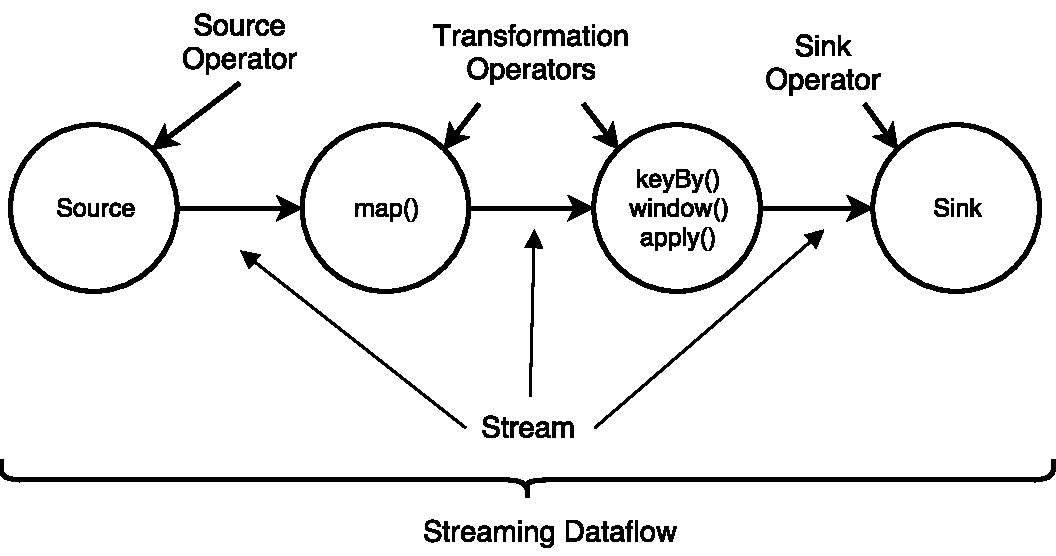
\includegraphics[scale=0.75]{Figures/dataflow.pdf}
	\decoRule
	\caption[Streaming Dataflow]{DAG outlining the previous code snippet}
	\label{fig:Dataflow}
\end{figure}

\paragraph{Event Time}

Flink supports different notions of time in streaming programs \cite{flink_eventtime}, each of them useful for specific use cases:

\begin{itemize}
    \item \textbf{Processing time} refers to the system time of the machine that is executing the respective operation.
    
    When it is being used, the system clock of the machines will be used to run all time-based operations. Being the simplest notion of time, no coordination is required between streams and machines, providing, this way, the best performance with the lowest latency. However, since the entire environment is distributed and might work asynchronously, processing time does not provide determinism, because of its susceptibility to the speed at which records arrive in the system and flow between each pair of operators inside the system.
    
    \item \textbf{Event time} is the time embedded within a record, representing when it occurred on its producing device. This time is typically assigned before records enter Flink and it can be extracted directly from the record at the Source level. An event time window of an hour will contain only records carrying an event timestamp within that hour, regardless of their actual time and order of arrival.
    
    Event time is especially useful when dealing with out-of-order or late events, and even on replays of data from persistent logs or backups. When using event time, the progress of time is discretized based on the data, rather than the clock, and the generation of the Event Time Watermarks, central to the mechanism that signals progress in event time,  must be specified internally to the program.
    
    Event time processing inherently causes a certain latency, due to its waiting for late and out-of-order events.
    
    \item \textbf{Ingestion time} is the time that events enter Flink. The source operator assigns to each record its current time as a timestamp, which all time-based operations refer to.
    
    Ingestion time can be considered an alternative, conceptually speaking, in between event time and processing time: it is more expensive than processing time, while providing deterministic results, as it uses stable timestamps assigned once at the source and used by all of the following time-based operations, but cannot handle any out-of-order events or late data, with respect to event time, even though there's no need to specify the watermarks generation.
\end{itemize}


\paragraph{Windows}

Windows are the core mechanism within a stream processing framework. They allow the application of operations after splitting the stream into \textit{buckets} of finite size. The structure of a windowed Flink program differs when considering \textbf{keyed} and \textbf{non-keyed} streams: a keyed stream is split into multiple logical sub-streams and a window is applied to each one of them separately, differently from a non-keyed stream where the window is applied globally and within a single task \cite{flink_windows}.

A Window lifecycle starts as soon as the first element belonging to it arrives, ending, by being completely removed, when the time, event or processing time, passes its end timestamp plus any user-specified \textbf{allowed lateness}. For example, in an event-time-based Flink application where a tumbling window is created every 5 minutes with an allowed lateness of 1 minute, a new window will be created for the interval between 11:30 and 11:35, as soon as a record with a timestamp falling into that interval arrives, and will be removed when the watermark passes the 11:36 timestamp.

For each window must be specified a \textbf{Trigger} and a function (\texttt{WindowFunction}, \texttt{ReduceFunction} or \texttt{FoldFunction}) attached to it: the Trigger is used to specify the conditions under which the window is considered ready or complete for the function to be applied, while the function will contain the operation to be applied to the contents of the window. The triggering policy is completely customizable and can even decide to purge a window’s contents, leaving the window metadata untouched, in order to add new data to that window.

It's possible specify an \textbf{Evictor}, used to remove elements from the window after the trigger fires and before and/or after the function is applied.

There are four main window assigners usable in Flink:

\begin{itemize}
    \item \textbf{Tumbling Windows} are fixed size and non-overlapping windows, configured with a parameter controlling how much frequently a new window has to be started.
    \item \textbf{Sliding Windows} are fixed size, similarly to tumbling windows, but are configured with an additional slide parameter, which controls how frequently a sliding window is started. Therefore they may overlap, with elements assigned to multiple windows.
    \item \textbf{Session Windows} group elements by sessions of activity. Session windows do not overlap and do not have a fixed start and end time, in contrast to tumbling windows and sliding windows. A session window closes when it does not receive elements for a certain period of time, i.e., when a gap of inactivity occurred.
    \item \textbf{Global Windows} assign all elements with the same key to the same single global window. This windowing scheme is only useful if you also specify a custom trigger. 
\end{itemize}



\paragraph{Parallelism} \label{ParallelismFlink}

Applications using Flink are inherently parallels and distributed. During execution, a stream may be divided in more than one partition; each operator can have more than a single sub-task operating on data, each one independent from the other and executed on different threads or, if possible, on different machines or containers.\\
The parallelism of a task is the parameter indicating the number of subtasks an operator can have and, consequentially, the number of partitions of the stream getting outputted from that operator.\\

\begin{figure}[!htb]
    \centering
    
\includegraphics[scale=0.75, trim=0.5cm 12cm 1cm 0.5cm]{Figures/parallel_dataflow.pdf}
    \decoRule
    \caption[Parallel Dataflow]{DAG with Parallelism=2}
    \label{fig:ParallelDataflow}
\end{figure}

Streams can transport data between a pair of operators following two different patterns: One-to-one pattern and redistributing pattern:
\begin{itemize}
	\item \textbf{One-to-one streams} preserve the stream partitioning and the order of the elements passed to the following operator. For example, the subtask[0] of a \texttt{map()} operator will get to see the same elements produced by the subtask[0] of the previous Source operator.
   
    \item \textbf{Redistributing streams} change their partitioning, sending the data to different subtasks, based on the transformation being applied. For example, a \texttt{keyBy()} operator repartitions the stream using the hash of the chosen key. In this case, the elements' order will be preserved only between neighbouring operations pairs, and won't be ever guaranteed being the same in the following operators.
\end{itemize}

\subsection{Data Streaming Fault Tolerance}

Flink offers built-in guarantees in case of failures, so that there's minimum disruption on the processing jobs and a consistent recovery of the data streaming applications' state. The two main features which allows recovery from errors or runtime exceptions are \textbf{Checkpoints} and \textbf{Savepoints}.

In case of a program failure (due to machine-, network-, or software failure), Flink stops the distributed streaming dataflow, restarting the operators and resetting them to the latest successful checkpoint, while also resetting the input streams to that same point of the state. Any records processed as part of the restarted parallel dataflow are guaranteed to not have been part of the previously checkpointed state.

For this mechanism to realize its full guarantees, the data stream source needs to be able to rewind the stream to a defined recent point. Apache Kafka, thanks to its offsets, has this ability and Flink’s connector to Kafka makes use of it.

\subsubsection{Checkpoints}

\begin{code}
    \label{code:checkpointing}
    \begin{minted}[breaklines, breakbefore=., breakafter=(]{Scala}
    val env: StreamExecutionEnvironment = StreamExecutionEnvironment.getExecutionEnvironment
    
    env.enableCheckpointing(60000)
    
    env.getCheckpointConfig.enableExternalizedCheckpoints(ExternalizedCheckpointCleanup.RETAIN_ON_CANCELLATION)
    
    env.setStateBackend(new FsStateBackend(state_dir, true)) 
    \end{minted}
    \captionof{listing}{An example of asynchronous checkpointing configuration on a FileSystem backend}
\end{code}~\\

\textbf{Checkpoints} are Flink's tool to guarantee automatic fault tolerance and recovery of the job's state, in case of runtime errors or failures \cite{flink_checkpointing}. 
\\
\\
They are, essentially, snapshots of the current state of the job that act consistently as the system fall back in case of failure. Flink’s mechanism for drawing these snapshots is inspired by the standard Chandy-Lamport algorithm \cite{Chandy:1985:DSD:214451.214456} for distributed snapshots and is specifically tailored to Flink’s execution model \cite{DBLP:journals/corr/CarboneFEHT15}. 
\\
\\
Checkpointing must be configured on the application level as shown in the previous snippet by calling the \texttt{enableCheckpointing(milliseconds)} to specify how much time should pass between two consecutive snapshots. By default, if a job is cancelled the checkpoint is deleted as well, so the retainment on cancellation must be enabled manually. 
\\
\\
An additional configuration available to application level setup is the State Back-end, that is the location where the checkpoint, thus, the job's state, should be saved. There are three possible back-ends which can be chosen from: \textbf{in Memory}, useful for testing, on a \textbf{Filesystem} (local or distributed, like HDFS) and on \textbf{RocksDB}\footnote{\href{http://rocksdb.org/}{RocksDB} is an embeddable persistent key-value store for fast storage}, particularly recommended for huge states. Optionally, snapshots can be taken asynchronously in order not to block the processing pipeline.
Checkpoints can be used to manually recover from failures through specific commands from Flink CLI, but they don't support scaling on recovery, that is, parallelism can't be changed when recovering from a snapshot.

\paragraph{Barriers}

A core element in Flink’s distributed checkpointing are the \textit{stream barriers}: lightweight elements flowing with the records, as part of the data stream, injected into the stream starting from the data source, without interrupting it. They are used to separate the records in the data stream belonging to two consecutive snapshots. Each barrier contains the ID of the snapshot whose records were pushed in front of it: there can be multiple barriers belonging to different snapshots, meaning that checkpoints may happen concurrently.
\\
\begin{figure}[!htb]
    \centering
    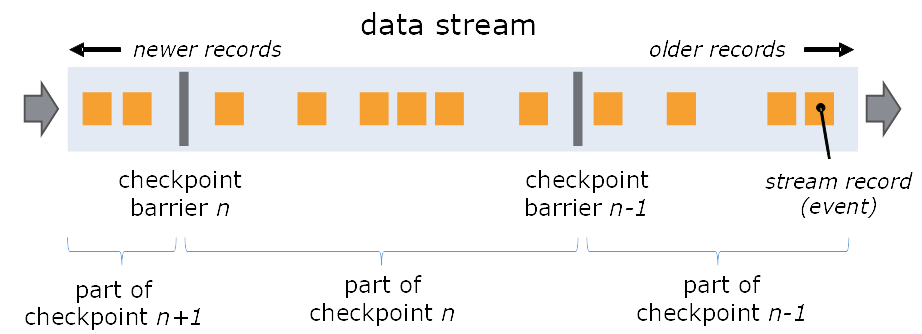
\includegraphics[width=1\linewidth]{Figures/stream_barriers}
    \caption{Visual representation of Stream Barriers}
    \label{fig:streambarriers}
\end{figure}
\\
Let's call $S_n$ the point in the stream where the barriers for snapshot $n$ are injected, representing the position up to which the snapshot covers the data, reported to the checkpoint coordinator, Flink’s JobManager.
\\\\
Flowing downstream, each intermediate operator must receive a barrier for snapshot $n$ from all of its input streams before emitting a barrier for the same snapshot into all of its outgoing streams, until a sink operator is reached. Once a sink has received a barrier $n$, from all of its input streams, the snapshot $n$ is acknowledged to the checkpoint coordinator and the checkpoint is considered complete.

At the completion of snapshot $n$, the job will never ask the sources to replay the records from before $S_n$, since they all went through the topology.
\\\\
If an operator receives more than one input stream, an \textit{\textbf{alignment}} step must be performed between all of the inputs:

\begin{itemize}
\item As soon as the operator has received a snapshot barrier $n$ from an incoming stream, it must wait the same barrier from all of the other inputs, since otherwise processing would mix records belonging to consecutive snapshots and, in this case, would use also the barriers for snapshot $n+1$.

\item While waiting, all barriers $n$ are temporarily set aside and the corresponding records put in an input buffer.
    
\item Once the last stream has received barrier $n$, the operator emits all pending outgoing records and then snapshot $n$ barriers itself, before continuing processing records, starting from input buffers and then the actual input streams.
\end{itemize}

\paragraph{Exactly Once vs. At Least Once}

The alignment step previously described may add latency to the streaming program, usually negligible, being in the the order of a few milliseconds, but some applications' latency may increase noticeably. If consistent super low latency (few milliseconds) for all records is a strict requirement, Flink allows to skip the stream alignment during a checkpoint, but snapshots are still drawn as soon as an operator has seen the checkpoint barrier from each input stream.

As a consequence, the operator keeps processing all inputs, including elements belonging to checkpoint $n+1$, which will then occur as duplicates when restoring the state of the stream because they are both included in the state snapshot of checkpoint $n$ and part of the data following this same checkpoint.
\\

The alignment step happens only when operators with multiple predecessors (join operators) or 
multiple senders (such as a stream repartitioning/shuffle) are present. For this reason, dataflows containing only parallel streaming operations (\texttt{map()}, \texttt{flatMap()}, \texttt{filter()}, …) guarantee \textit{exactly once} semantics even in \textit{at least once} mode.

\subsubsection{Savepoints}

\begin{code}
    \label{code:savepoint}
    \begin{minted}{Bash}
flink savepoint <jobId> [<savepointDirectory>] -yid <yarnAppId> 
    \end{minted}
    \captionof{listing}{Savepoint triggering from the Flink CLI}
\end{code}~\\

\textbf{Savepoints}, just like checkpoints, serve the purpose to save the state of a Flink application in case of cancellation or failures. Differently from checkpoints, they can only be performed manually from the Flink CLI, but support parallelism rescaling and they're the go-to choice when Flink's application computational capabilities must be improved by setting an higher parallelism factor or when an upgrade to a more recent version of Flink must be performed. Savepoint's mechanism works such that it associates each application's stateful operator, to its own state in a map-like structure: for this very reason, in order to successfully preserve state when upgrading a Flink application, each stateful operator needs to have its own \texttt{uid} set.

\subsection{High Availability}

A Flink's setup, whether a standalone cluster (being it containerized or physical) or using Distributed Resource Managers such as \nameref{YARN} or Mesos, is made of a Job Manager and one or more Task Managers, each one with one or more parallelism slots (cores usable for processing). Task Managers (TMs) handle jobs actual executions, while the Job Manager (JM) handles TM orchestration and monitoring and, for this reason, is a single point of failure, whose crash causes the entire Flink cluster to stop.
Flink High Availability setup follows the principles of a Active-Standby architecture (also used by HDFS Namenode e YARN Resource Manager HA set-ups) where a single leading JM is active, while multiple JMs standby, ready to take over leadership in case the leader failure. This guarantees that there is no single point of failure and programs can make progress as soon as a standby JM has taken leadership. There is no explicit distinction between standby and master JM instances: all of the possible JMs are registered as masters to \textbf{Zookeeper}, which is going to handle failure scenarios.

In case of YARN clusters configured in High Availability mode, a single JM, the \textbf{Application Master}, is run, but YARN itself will restart its container on failures. As additional configuration, the maximum number of attempts for the application masters needs to be configured in the YARN configuration.

\subsection{Flink Extensions} \label{FlinkLibs}

\subsubsection{FlinkCEP: Complex Events Processing}

FlinkCEP is a Flink extension adding the possibility to analyse events pattern in a DataStream, thanks to the Pattern API. This API allows the definition of patterns to be found in a stream and their selection in order to create a new DataStream of Alerts.\\


\begin{code}
\label{code:pattern-example}
\begin{minted}[breaklines]{Scala}

val inputStream: DataStream[SensorEvent] = ...

val pattern = Pattern.begin("start").where(_.getId == 42)
.next("middle").subtype(classOf[TemperatureEvent]).where(_.getTemperature >= 90.0)
.followedBy("end").where(_.getName == "end")

val patternStream = CEP.pattern(inputStream, pattern)

val result: DataStream[Alert] = patternStream.select(createAlert(_))
\end{minted}
\captionof{listing}{An example of Pattern API usage}
\end{code}~\\

In FlinkCEP, a \textbf{Pattern}, similarly to a pattern of a Regular Expression, can be \textbf{single} or \textbf{iterative}. For example, in a pattern like \texttt{"a b+ c? d"}, \texttt{a}, \texttt{c?} e \texttt{d} are single patterns, while \texttt{b+} is iterative.
\\
In a Pattern there can be, analogously to regular expressions, \textbf{quantifiers} and \textbf{conditions}.

\paragraph{Quantifiers}

Iterative patterns can be specified with the following self explanatory methods:

\begin{itemize}
    \item \texttt{pattern.oneOrMore()};
    \item \texttt{pattern.times(\#ofTimes)};
    \item \texttt{pattern.optional()}
\end{itemize}

\paragraph{Conditions}

Each pattern can have additional conditions specified, which can be related to a property of an incoming event, or the contiguity to other events.

Methods \texttt{pattern.where()} and \texttt{pattern.or()} can be used to specify \texttt{\justify{IterativeCondition}}s, \texttt{SimpleCondition}s or a combination of multiple conditions. In this case, combinations can be specified concatenating all the previous methods, including the quantifiers, optionally adding more constraints on the contiguity of the same pattern by calling \texttt{consecutive()}, for the strict contiguity, and \texttt{allowCombinations()} for the relaxed non-deterministic contiguity.
\\
Some examples:

\begin{code}
\label{code:iterative-cond}
\begin{minted}[breaklines]{Scala}
middle.oneOrMore().where(
    (value, ctx) => {
        lazy val sum = ctx.getEventsForPattern("middle")
                          .asScala.map(_.getPrice).sum
        value.getName.startsWith("foo") && sum + value.getPrice < 5.0
    }
)
\end{minted}
\captionof{listing}{Iterative Condition}
\end{code}~\\

\begin{code}
    \label{code:simple-cond}
    \begin{minted}[breaklines]{Scala}
//Example of conjunction through where concatenation
start.where(event => event getName startsWith "foo" ) )
     .where(event => event getTotal equals 50  )

start.subtype(classOf[SubEvent]).where(subEvent => ... /* some condition */)
    \end{minted}
    \captionof{listing}{Conditions combinations}
\end{code}~\\

\paragraph{Pattern Combination}

Similarly to conditions combination, pattern combination is possible through the consecutive calls to the following methods allowing to specify the contiguity constraints which a given pattern should satisfy:

\begin{itemize}
    
    \item \texttt{next()}, for strict contiguity.
    \item \texttt{followedBy()}, for relaxed contiguity.
    \item \texttt{followedByAny()}, for non deterministic relaxed contiguity.
    \item \texttt{notNext()}, NOT pattern with strict contiguity.
    \item \texttt{notFollowedBy()}, NOT pattern with relaxed contiguity.

\end{itemize}

Each pattern combination can be followed by a time constraint specified by concatenating \texttt{within(Time)}.

\paragraph{Pattern Detection}

Once a pattern sequence has been specified, it needs to applied to the target \texttt{Datastream}, creating this way a \texttt{PatternStream}.
On this new stream \texttt{select} or \texttt{flatSelect} operations need to be applied in order to enable further processing on the events satisfying the pattern.

\subsubsection{Other extensions: Flink Gelly and FlinkML}

In addition to the aforementioned library for complex event handling, Flink makes available specific sets of API, which provide useful tools when it comes to enable advanced processing on data.

\paragraph{Flink Gelly} is an API based on the Flink \texttt{Dataset}s API specifically developed for Graph Processing. Graphs are stored as a finite set of vertices and edges, a special case of a \texttt{Dataset}. This library allows the application of operators like Map, Filter, Intersect and Union, mutations like edge and vertex removal, but also advanced techniques belonging to Graph Theory like \textit{Iterative Graph Processing} (Vertex-centric, Scatter-Gather and Gather-Sum-Apply), \textit{Single Source Shortest Paths}, \textit{Clustering} and \textbf{Similarity Analysis}.

\paragraph{FlinkML} is a set of tools which allows the application of Machine Learning techniques over Flink data sets, including both algorithmic implementations for supervised (\textit{SVMs} and \textit{Multiple Linear Regressors}) and unsupervised (\textit{K-nearest neighbours}) learning, Data Preprocessing and Recommendation (\textit{ALS}).


